
\documentclass[10pt, conference, compsocconf]{IEEEtran}

\usepackage{graphicx,algorithmic}
\usepackage{url}
\usepackage{amssymb,subfigure}
\hyphenation{op-tical net-works semi-conduc-tor}
\newcommand{\etal}{\emph{et al. }}
\newcommand{\R}{\mbox{$\mathbb{R}$}}
\begin{document}


\title{Data Mining in Wind Energy Information Systems with WindML}



\author{Submitted for Blind Review\\Institute Address}


\maketitle


\begin{abstract}
The challenge of processing large data sets with data mining techniques has arrived smart energy grids. Wind energy is playing an increasingly important part for ecologically friendly power supply. The fast growing infrastructure of wind mills can be viewed as large sensory system screening the wind energy with high temporal resolutions. The resulting large data bases of wind energy time series can be used for prediction, control, and planning. In this work, we describe WindML, a framework and collection of wind energy data mining algorithms-based on python and scikit-learn. Our goal is the continuous development of machine learning tools to address the challenges of a growing wind energy information infrastructures. In this paper, we introduce three examples and use-cases that demonstrate typical functions and modules of WindML.
\end{abstract}

\begin{IEEEkeywords}
wind energy, wind prediction, ramp detection, classification, regression, dimensionality reduction

\end{IEEEkeywords}


\IEEEpeerreviewmaketitle



\section{Introduction}

The importance of wind in smart grids with a large number of small renewable energy resources is increasing. With the growing infrastructure of wind turbines and the according availability of time series data with high spatial and temporal resolution, the application of data mining techniques comes into play. For example, one data set we employ in our study consists of more than 240 GB of data of more than thirty thousand turbines over three years in a 10-minute resolution. This high spatial and temporal resolution offers the chance for successfully mining precise knowledge for prediction, planning, and optimization, e.g., for a stable integration of wind energy. With efficient and specialized data mining techniques that extract knowledge from the large wind data bases, it is now possible to solve prediction and planning problems. This paper introduces WindML, a machine and data mining learning library for wind energy information systems. The goal of WindML is to offer specialized techniques and and easy to data-mining and machine learning methods based on Python and scikit-learn. Classification, regression, clustering, and dimensionality reduction methods allow to solve planning and optimization problems. It is based on the western wind data set of the \textit{national renewable energy laboratory} (NREL). 

A related python and scikit-learn framework has been introduced for astronomical data sets. AstroML integrates machine learning and data mining techniques into astronomical data sets and is mainly based on the sloan digital sky survey (SDSS)~\cite{sdss} data.


The paper is structured as follows. In Section~\ref{sec:data}, we introduce the framework and the data sets our analysis is based on. Section~\ref{sec:pred} concentrated on the prediction of wind energy. In Section~\ref{sec:ramps}, we introduce a ramp prediction module that treats the detection of wind energy ramp events as classification problem. Section~\ref{sec:dimred} introduces a dimensionally reduction module that allows visualization of high-dimensional wind time series data. Future work is sketched in Section~\ref{sec:cons}.



\section{Framework and Data Sets}
\label{sec:data}

The WindML framework allows the integration of arbitrary wind time series data sets~\cite{astroML}. It is based on the machine learning and data mining methods of scikits-learn and ...
todo: Justin!


\subsection{Framework Background}

todo: Justin!
WindML is...
- based on scikits-learn....github...
- implements easy-to-use method for loading data and building patterns
- data is (successively?) loaded from WindML server when needed
- documented reference
- documented, downloadable examples with text and graphical output on website (url!)


\subsection{NREL Data}

Currently, the framework employs the \textit{western wind data set} of the \textit{national renewable energy laboratory} (NREL), which comprises three years of wind energy time series data. The NREL data set consists of wind energy time series data of 32,043 wind turbines, each holding ten 3\,MW turbines over a timespan of three years in 10-minute resolution. The data is based on a numerical weather prediction model, whose output has been modified with statistical methods in such a way, that the ramping characteristics are more comparable with those observed in reality~\cite{Potter}. Figure~\ref{fig:screen} shows an example screenshot of the NREL user interface that allows browsing and downloading of the NREL wind turbine data sets. Figure~\ref{fig:cor} illustrates the correlations between the energy time series of neighbored wind turbines and a target turbine one time step ahead. The figure has been generated with the WindML correlation module and is part of the WindML statistics and visualization toolkit. The statistics module also comprises methods for generating features from wind time series, statistical surveys of wind, power, ramps and other properties as well as methods for visualization of time series and topographical characteristics.



\begin{figure}[h]
\centering
\subfigure[\label{fig:screen}screenshot NREL]{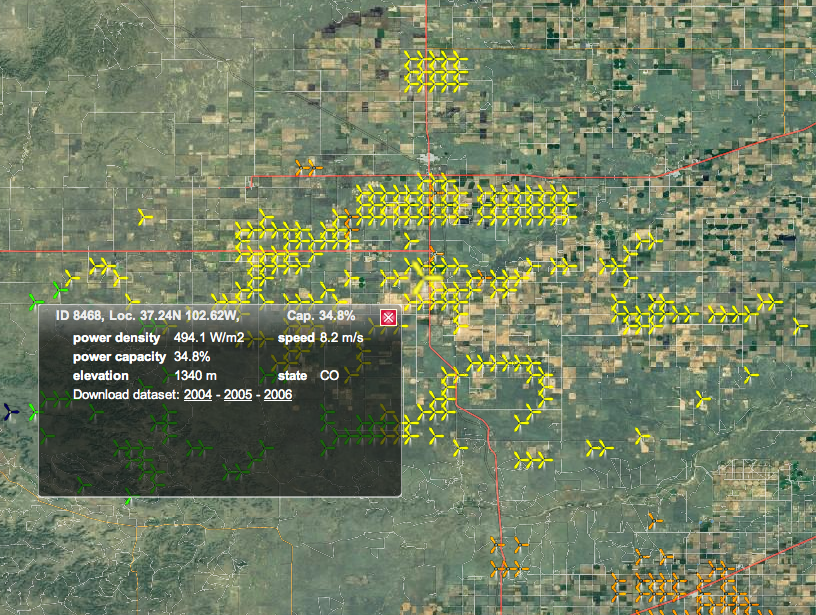
\includegraphics[scale=0.16]{pics/map.png}}
\subfigure[\label{fig:cor}correlations of energy]{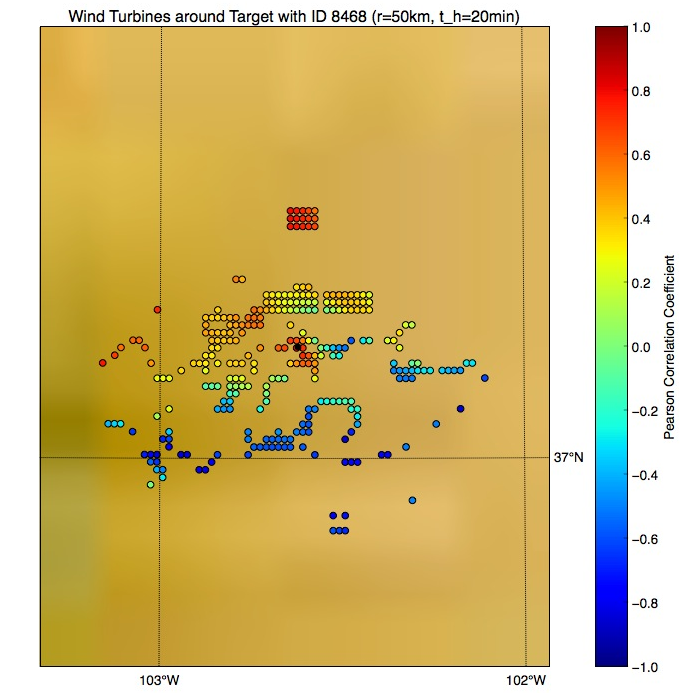
\includegraphics[scale=0.15]{pics/corr.png}}
\caption{(a) Screenshot of visual NREL user interface for browsing wind energy data at turbine with ID = 8468, (b) correlation of wind energy time series between neighbored turbines and target turbine.}
\label{fig:park}
\end{figure}



\section{Prediction of Wind Energy: A Comparison of Regression Methods}
\label{sec:pred}
\subsection{General Time Series Model}
In this section we employ statistical wind power predictions for short term forecasts of the energy production of a turbine. Thereby, our model makes predictions exclusively with the past measurements by formulating the prediction task as regression problem. \\
Let us first assume, that we consider the times series of a single turbine, which production we want to predict. The wind power measurement $x(t)$ is mapped to the power production at a later time \mbox{$y = x(t\!+\!t_h)$}. It is also conceivable to take past observations $x(t\!-\!1), x(t\!-\!2), \cdots, x(t\!-\!\mu)$ with $\mu \in \mathbb{N^+}$ and the changes
of the measurements \mbox{$\Delta x_{1} = x(t)-x(t\!-\!1), \cdots, \Delta x_{\mu}=x(t\!-\!(\!\mu\!-\!1))-x(t\!-\!\mu)$} into account. Considering all this, we get the following mapping:  $\mathbf{X} = [x(t), x(t\!-\!1), \cdots, x(t\!-\mu), \Delta x_{1}, \cdots, \Delta x_{\mu}]{}^{T} \longrightarrow y=x(t\!+\!t_h)$.
In this way, patterns $\mathbf{X}$ of the high dimensional feature space $\mathcal{X} \subseteq \mathbb{R}^d$ with \mbox{$d=(2\mu+1)$} are projected in a target value $y$ of the 1-dimensional label space $\mathcal{Y} \in \mathbb{R}$. With the presence of a set $T$ of $N$ training pairs \mbox{$T=\{(\mathbf{X}^1,y^1),\ldots,(\mathbf{X}^n,y^n)\}$}, one has to find an optimal function $f: \mathcal{X} \rightarrow \mathbb{R}$ that provides good predictions to unseen patterns $\mathbf{X} \in \mathcal{X}$.

\subsection{Details of Evalutation}
In our folowing examples we train three various regression models with a 2-fold cross-validation on fist half of year 2006. The second half is used for evalution by determining the square error of the forecasts $p_f^i$ with the measured power outputs $p_m^i$: \,\,  $L_2\,(p_m, p_f) = \sum_{i=t_{start}}^{t_{end}}\big(p_{f}^i-p_{m}^i\big)^2$.  
For the comparison of the regression models we consider $\mu=2$, i.e., 3 features of the times series (2\,power outputs and their difference). 

\subsection{Linear Regression}
First, we employ the a linear regression model, based on ordinary least squares method. 



\section{Classification of Wind Energy Ramp Events}
\label{sec:ramps}

A critical issue in maintaining grid stability are sudden and large changes (up and down) of wind power, which are called ramp events. In this section, we introduce the wind power ramp event prediction module. After the definition of ramp events, we define the ramp event prediction problem as classification problem and introduce the ramp separation and the ramp detection application case. In the experimental part, we concentrate on three reference turbines, i.e., in Tehachapi (CA, ID 4155), in Palm Springs (CA, ID 1175) and a turbine near Reno (NV, ID 11600).


\subsection{Ramp Event Definition}

In literature, ramps are not clearly defined \cite{kamath,focken} and may vary in location and sizes of wind farms and turbines. We define a ramp events as follows. Let $\mathbf{x}(t)$ be the wind time series of a wind park, and let $y(t)$ be the time series of the target turbine, for which we determine the forecast. A ramp event is defined as a wind energy change from time step $t$ to time step $t+\alpha$ by $\theta \in (0, y_{\max}]$, i.e., for an ramp-up event, it holds $y(t+\alpha) - y(t)>\theta$, for a ramp-down event it holds $y(t+\alpha) - y(t)<-\theta$. 

Figure~\ref{fig:ramps} visualizes the differences of time series of our test wind turbine in Tehachapi. The wind energy $y(t)$ at time $t$ is plotted against the energy at time $t+\alpha$. If the wind does not change, dots are plotted on the main diagonal. Stable wind situations, i.e., dots near the main diagonal, occur more often than larger wind changes. Ramp events are comparably rare. The number of ramps increases with the time horizon\footnote{This holds for small time horizons, as a ramp-down may be followed by a ramp-up event over a larger horizon.} $\alpha$, as a ramp event may appear multiple times.

\begin{figure}[thb]
\centering
\subfigure[$\alpha = 1$]{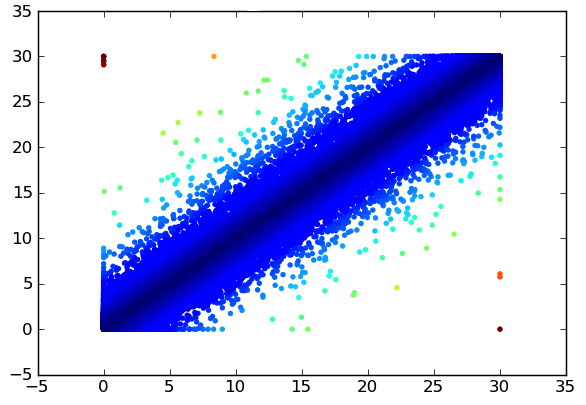
\includegraphics[scale=0.2]{pics/r1.png}}
\subfigure[$\alpha = 2$]{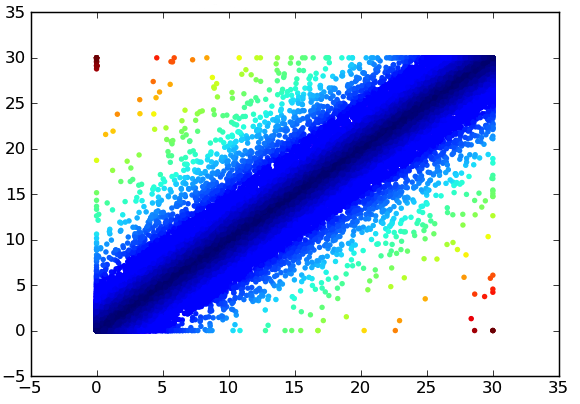
\includegraphics[scale=0.2]{pics/r2.png}}
\caption{Plot of wind energy changes of reference turbine in Tehachapi for two time steps.}
\label{fig:ramps}
\end{figure}



\subsection{Related Work on Statistical Learning and Ramp Events}

Most related work in ramp event prediction is based on numerical weather prediction (NWP) models~\cite{greaves,focken}. %a survey is given in~\cite{ramp_survey}. 
Only few approaches concentrate on forecasts based on data mining methods. Zareipour \etal~\cite{svm_ramp} analyze the recognition of ramps on the Albert wind power data set that consists of wind time series data from a park near the Rocky Mountains. The model takes into account univariate input variables and neglects the problem of unbalances data sets.


% The model is not based on the wind measurements from turbines in the environment. In the experimental part, four classes are employed (-300 to 50, -50 to 0, 0 to 50 and 50 to 300). The employed error measurement is based on classification accuracy. The problem of unbalanced data sets is not taken into account.


\subsection{Ramp Event Prediction as Classification}

We define the ramp prediction problem as the task to predict, whether a ramp-up or a ramp-down event starts at time $t$, i.e., an energy change from time $t$ to time $t+\alpha$. This problem can be defined as classification problem. We can understand any agglomeration of wind measurements $y(t),y(t-1),\ldots$ at present and in the past of the target turbine, and for any surrounding turbine $x_n(t)$ for $n \in \mathcal{N}$ in the set $\mathcal{N}$ of neighbored turbine as pattern $\mathbf{x}_i=\mathbf{x}(t)$. The ramp event serves as label (e.g., $0$ for no-ramp, $1$ for ramp-up, and $2$ for ramp-down). Figure~\ref{fig:park} shows the construction of a pattern $\mathbf{x}_i$ based not on the radius $r$ around the target turbine.

If we have observed a training set of such observations, i.e., $\{ (\mathbf{x}_i, y_i) \}_{i=1}^N$, we train a classifier and predict the ramp for an unknown observation (pattern respectively) $\mathbf{x}'$. In the experimental sections, we will employ and SVM as classifiers. An alternative kind of way to predict ramps is to treat the problem as regression problem by determining ramps of the continuous power prediction of a target turbine.

Besides the classifier accuracy (square loss), we will employ two quality measures to evaluate the quality of a ramp prediction method. Let $f_t$ be the number of true forecasts, $\tau$ the number of false forecasts, and $r_m$ the number of missed ramps, then $f_a = f_t/(f_t+\tau)$ is the forecast accuracy and $r_c = f_t/(f_t+r_m)$ the ramp capture. The forecast accuracy $f_a$ is an indicator for the ability of the model to determine the correct label of a pattern.


\subsection{Ramp Separation}

As first step, we learn a classifier that separates ramp-up from ramp-down events. For our reference turbines, ramp-up and ramp-down events of different heights $\theta = 15$ are detected. Table~\ref{tab:1} shows the number of ramp events for each data set. We define a pattern as the wind energy of the neighbored turbines and the reference turbines within a radius of $r=10$ km at time $t$ and $t-1$. Corresponding labels are ramp-up and ramp-down events.


\begin{table}
\small
\vspace{-0.5cm}
\caption{\label{tab:1}Ramp classification: ramp-up vs. ramp-down and classification accuracy, $\alpha = 2$.}
\begin{center}%
	\begin{tabular}{| l | l | l | l |l | l | l |l |l |}
\hline
loc.	&  height & $d$ & up & down & no  & MSE \\
\hline
teha & 10  & 132& 139 & 93 & 0 & 0.93\\ % RBF, C= 1000, gamma=1e-06
teha & 15 & 132&  50 & 42 & 0 & 0.96\\ % RBF, C= 10, gamma=1e-05
\hline
palm & 10  & 84&  140 & 90 & 0 & 0.92\\ % rbf C=100, gamma=1e-05
palm & 15 & 84& 48 & 20 & 0 & 0.95\\ % rbf, C= 1000, gamma 1e-06
\hline
reno & 10  & 120& 158 & 168 & 0 & 0.90\\ %C = 0.01 linear
reno & 15 &  120 & 48 & 56 & 0 & 0.98\\  % rbf, C = 10, gamma=1e-05
\hline
\end{tabular}
\end{center}
\end{table}


The support vector machine (SVM) is trained with grid search and 5-fold cross-validation on half of the data set. As parameterizations, a linear kernel with $C \in \{ 10^{-10}, \ldots, 10^{20} \}$ and the RBF kernel with settings $\sigma, C \in \{10^{-10}, \ldots, 10^{20} \}$ are tested. The other half of the data is employed for evaluation. The experimental results are summarized in Table~\ref{tab:1} showing the classification accuracy w.r.t. MSE. The results show that the classifiers are able to distinguish between ramp-up and ramp-down events with a high accuracy.


\subsection{Recognition of Ramps}

We enhance the classification problem to a three class problem considering no-ramp patterns. We employ the same settings like in the previous section, i.e.f, 5-fold cross-validation and the search in the parameter space specified above. Table~\ref{tab:2} shows the description of training and test set and the experimental results. The classifier accuracy decreases to values between 0.65 and 0.76. But the forecast accuracy $f_a$ is comparatively high with values over $0.8$ and up to $0.9$. The results for ramp capture depend on the turbine location. For Tehachapi, better ramp capture results are achieved than for Palm Springs and Reno.


\begin{table}[h]
\small
\caption{\label{tab:2}Ramp classification: ramp-up vs. ramp-down vs. no-ramps and classification accuracy.}
\begin{center}%
	\begin{tabular}{| l | l | l | l |l | l | l |l |l |l |l |l |l |l |l |l |}
%\hline
%& & &  r_clticolumn{6}{c|}{$\alpha = 1$}\\
\hline
loc.	&  $\theta$ & d & up & down & no  & MSE & $f_a$ & $r_c$  \\
\hline
teha & 10  & 132 & 40 & 28 & 75 & 0.76 &0.81 & 0.77 \\
teha & 15 & 132 &  13 & 13 & 28 & 0.74 & 0.82 & 0.88  \\ % a
\hline
palm & 10  & 84 & 38 & 18 & 54 & 0.75 & 0.86 & 0.64  \\
palm & 15 & 84 & 13 & 3 & 14 & 0.73 & 0.90 & 0.63 \\
\hline
reno & 10  & 120 & 50 & 55 & 78 & 0.65 & 0.82 & 0.58  \\
reno & 15 & 120 & 10 & 13 & 32 & 0.73 & 0.87 & 0.62  \\
\hline
\end{tabular}
\end{center}
\end{table}


The standard model employs all turbines in a specified radius to construct a pattern. To answer the question, if a subset of features can improve the prediction, we employ the scikit-learn implementation of recursive feature elimination (RFE) for a linear SVM. Figure~\ref{fig:features} shows cross-validation score using RFE with a linear SVM and 2-fold cross-validation for two turbines, i.e., (a) in Palm Springs, and (b) in Reno for two ramp heights and prediction horizons w.r.t. a varying number of features, which have been recursively eliminated from the learning setting. The error is decreasing with increasing number of features. In the Palm Springs example, the error is minimal as of about 65 features, in Reno already as of 20 features. For a short time horizon of $\alpha=1$, better accuracies can be achieved.

\begin{figure}[thb] % generated with feature.py
\centering
%\subfigure[Tehachapi]{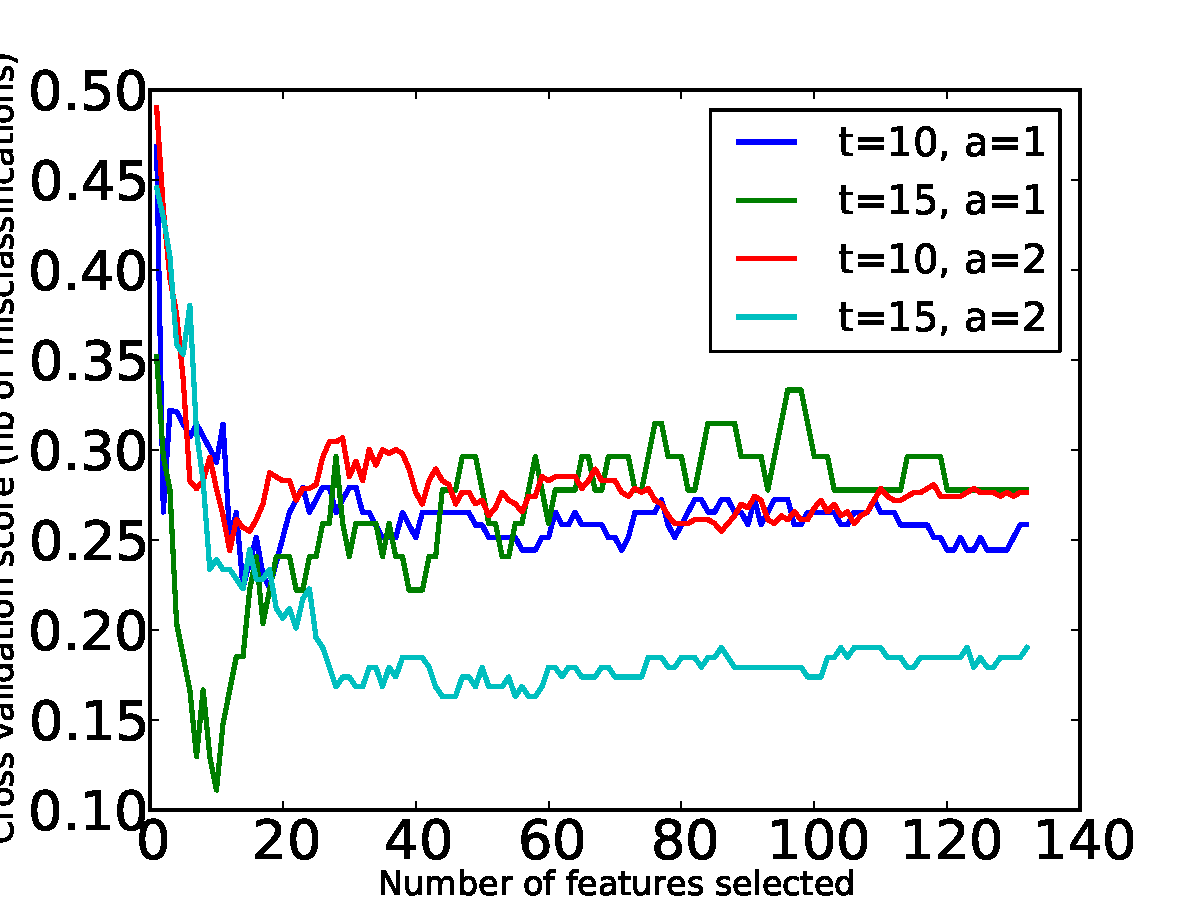
\includegraphics[scale=0.2]{pics/teha.pdf}}
\subfigure[Palm Springs]{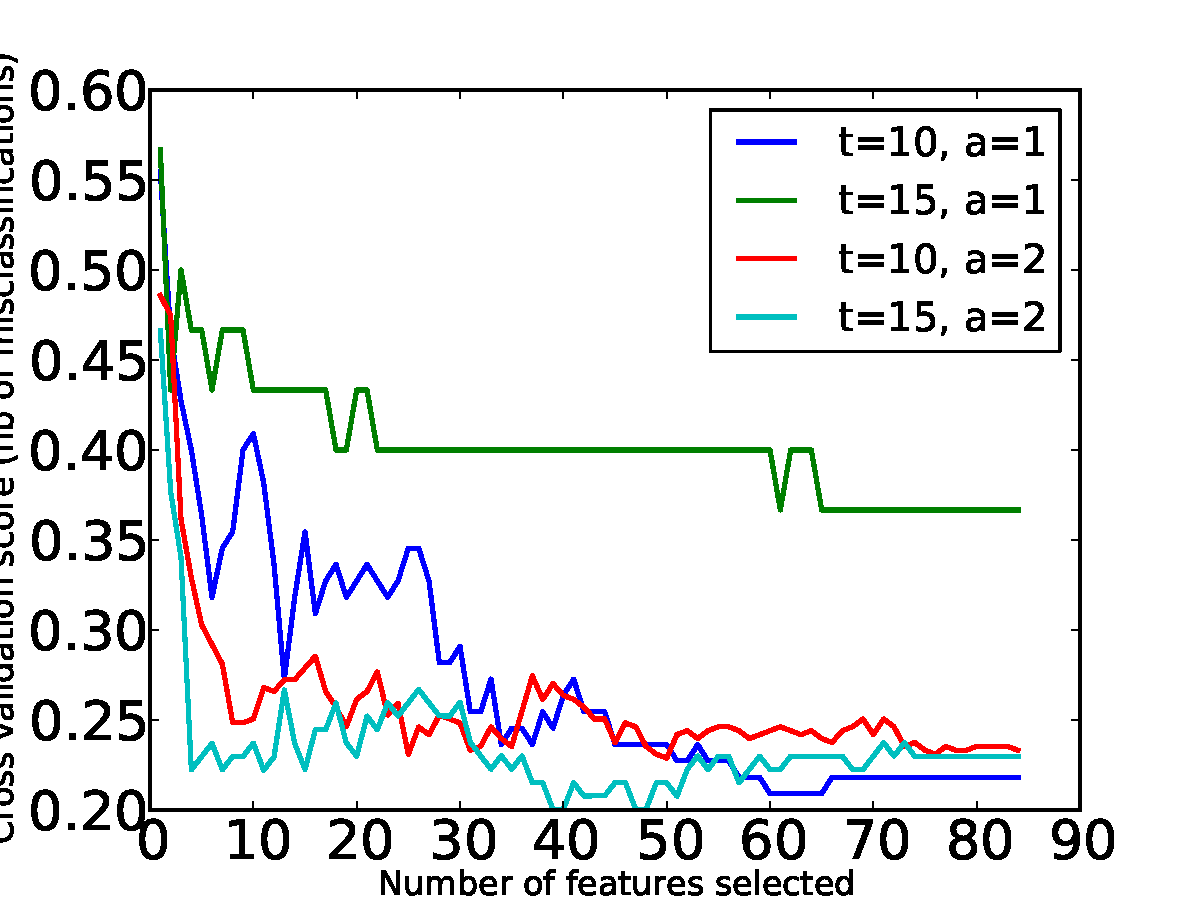
\includegraphics[scale=0.2]{pics/palm.pdf}}
%\subfigure[Palm Springs]{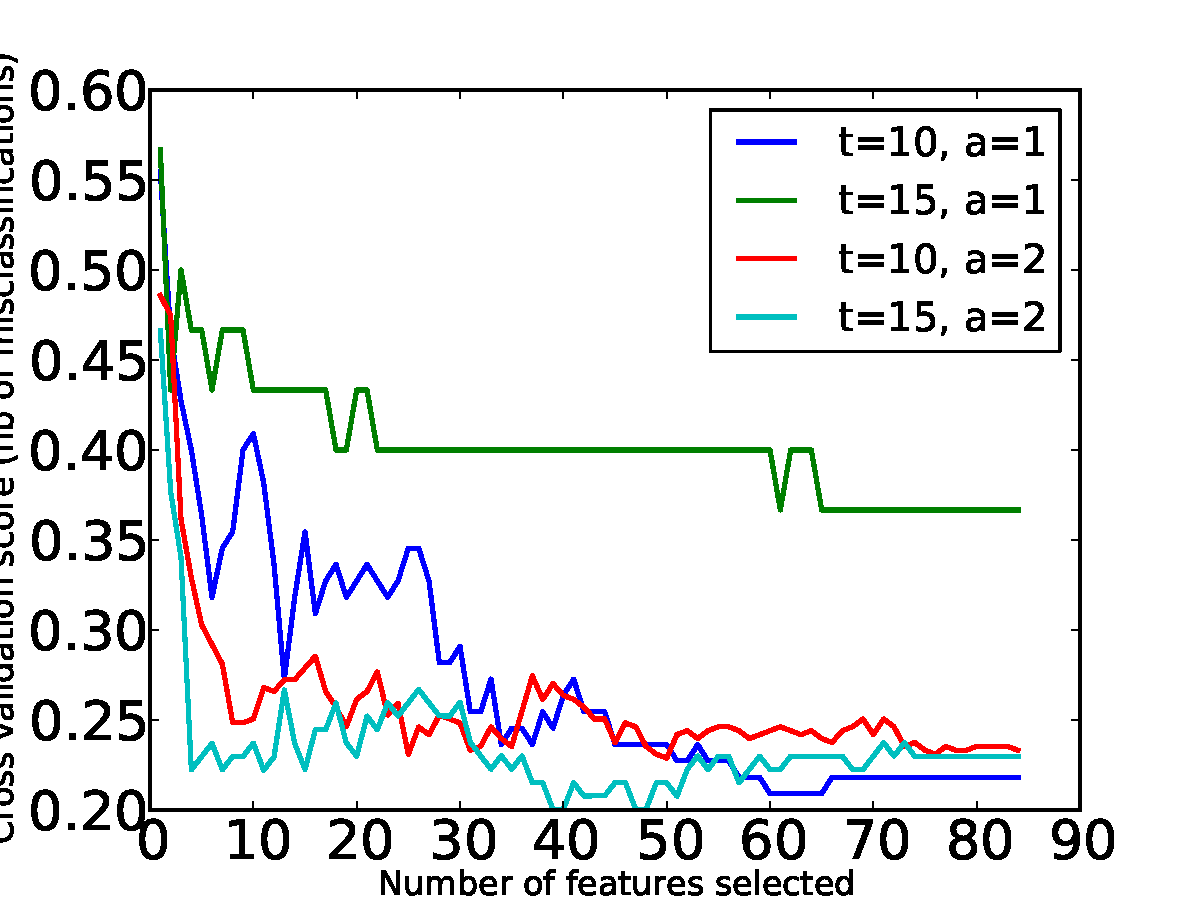
\includegraphics[scale=0.2]{pics/palm.pdf}}
\subfigure[Reno]{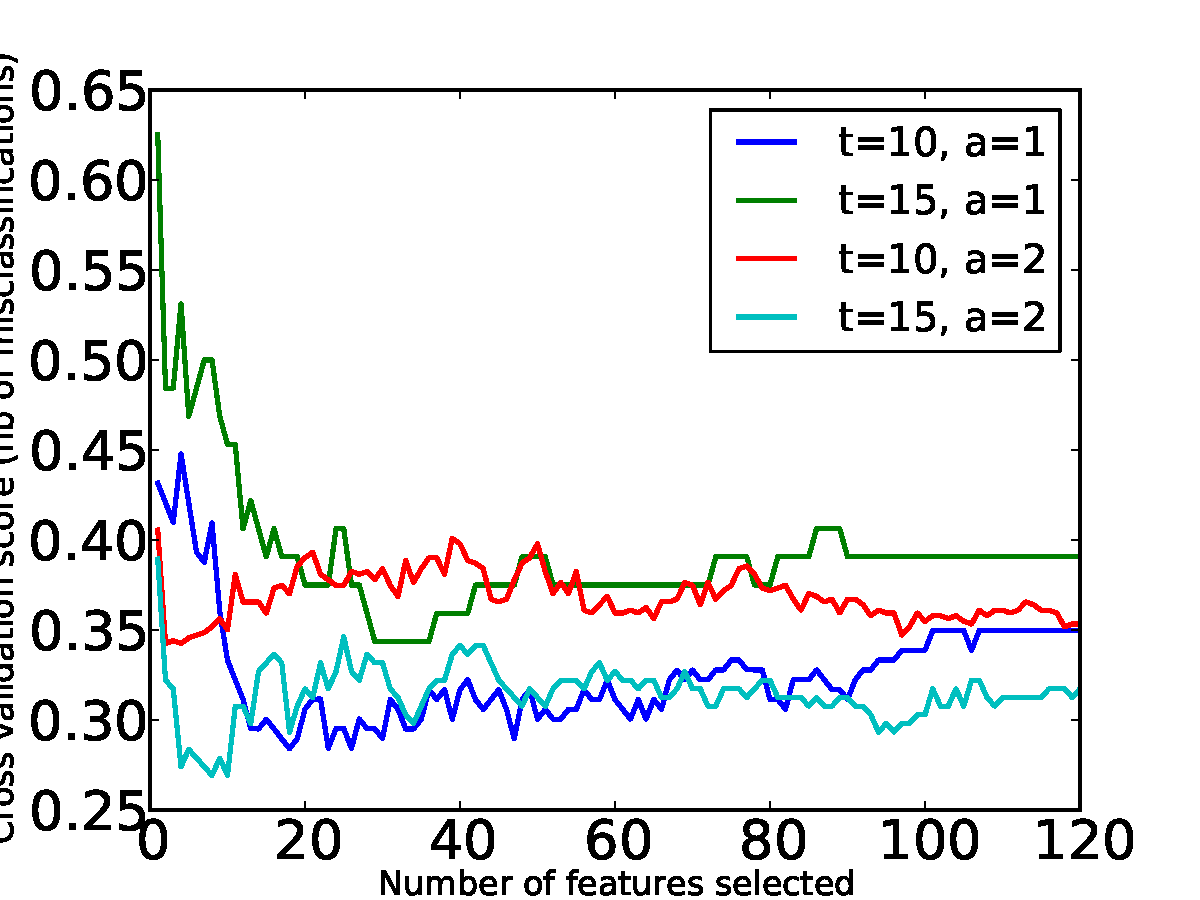
\includegraphics[scale=0.2]{pics/reno.pdf}}
\caption{Recursive feature elimination, i.e., tuning of selected features with a linear SVM and 2-fold cross-validation for (a) Palm Springs, and (b) Reno for $\theta = 10,15$ and $\alpha = 1,2$.}
\label{fig:features}
\end{figure}




\subsection{Imbalanced Training and Test Sets}

The balance of labels in training and test set significantly influences the learning and the evaluation result. For prediction of wind ramp events, this effect has an important implication for the ramp event prediction problem. First, we illustrate the imbalance problem for a classifier trained on a balanced training set, predicting the labels on an imbalanced set. Figure~\ref{fig:unbalanced1} shows the corresponding results for (a) Reno and (b) Palm Springs. The ramp capture result $r_c$ is independent of the number of no-ramp patterns, as no-ramp patterns do not affect the number of true forecasts $f_t$ and the number of missed ramps $r_m$, when only increasing the number of no-ramps. The accuracy score of the classifier increases, as the precision on the no-ramp events is relatively high, i.e., increasing from 0.91 to 0.98. But we can observe that the forecast accuracy drops out significantly. The reason is that the number of false forecasts is dramatically increasing, e.g., from 34 to 556.

\begin{figure}[thb]
\centering
\subfigure[Tehachapi, $\theta = 15, \alpha = 1$]{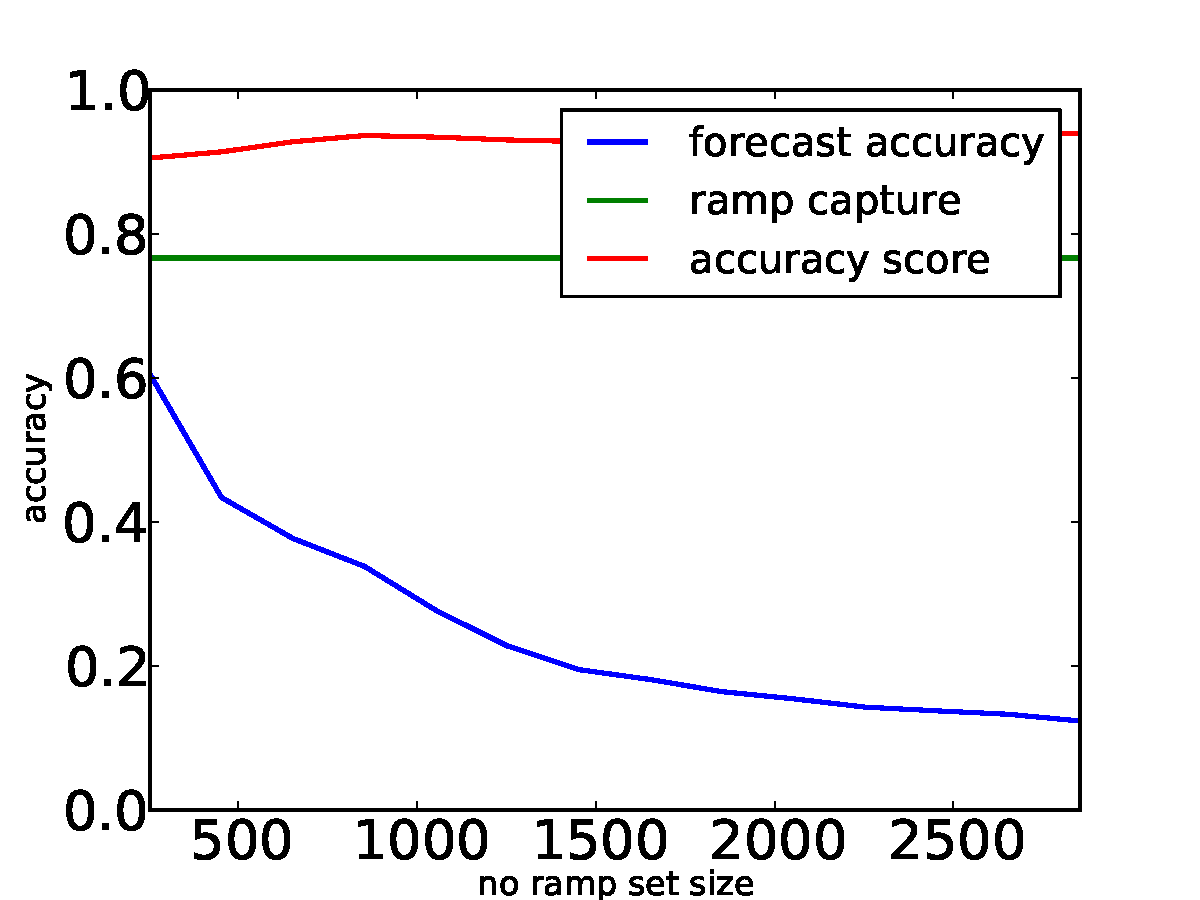
\includegraphics[scale=0.2]{pics/teha_test_h15_a1.pdf}}
%\subfigure[Tehachapi, $\theta = 10, \alpha = 2$]{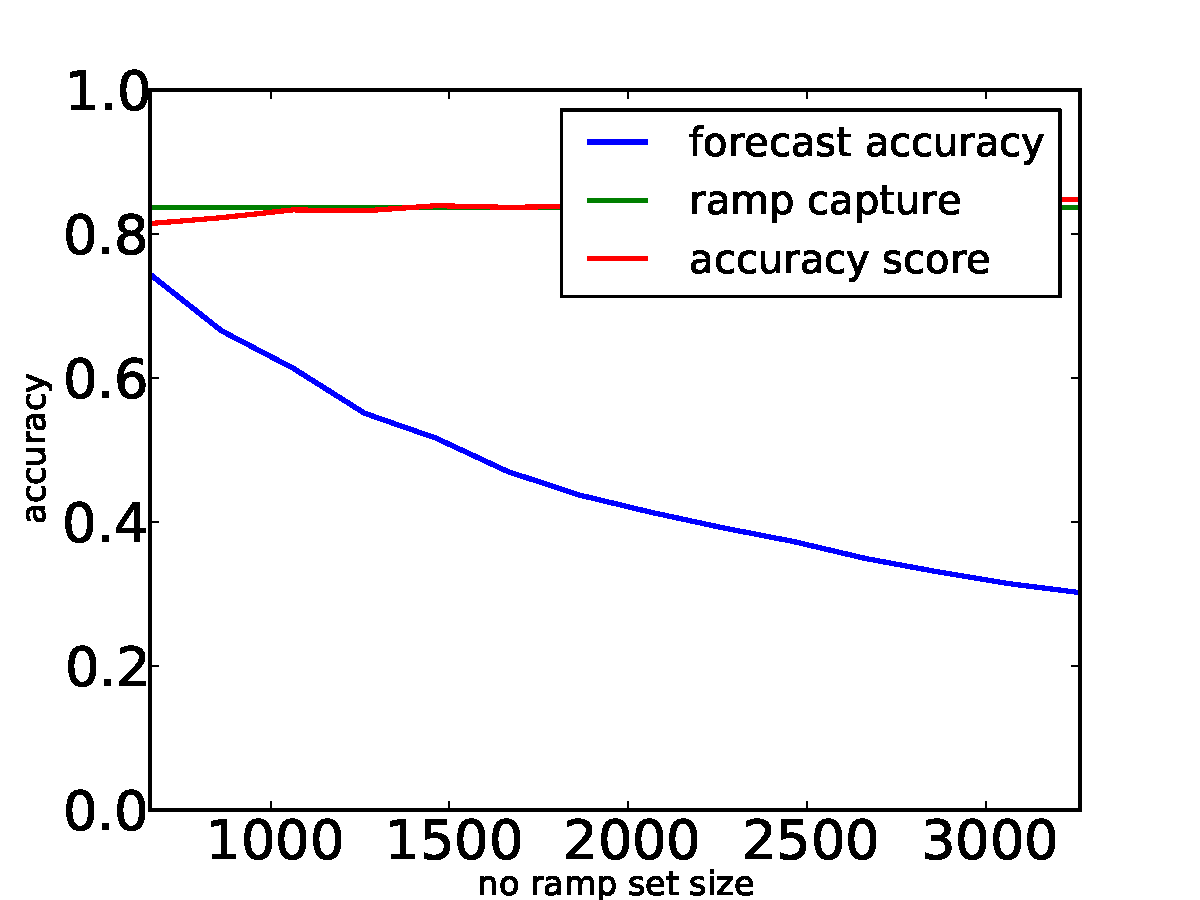
\includegraphics[scale=0.2]{pics/teha_test_h10_a2.pdf}}
%\subfigure[Reno, $\theta = 15, \alpha = 1$]{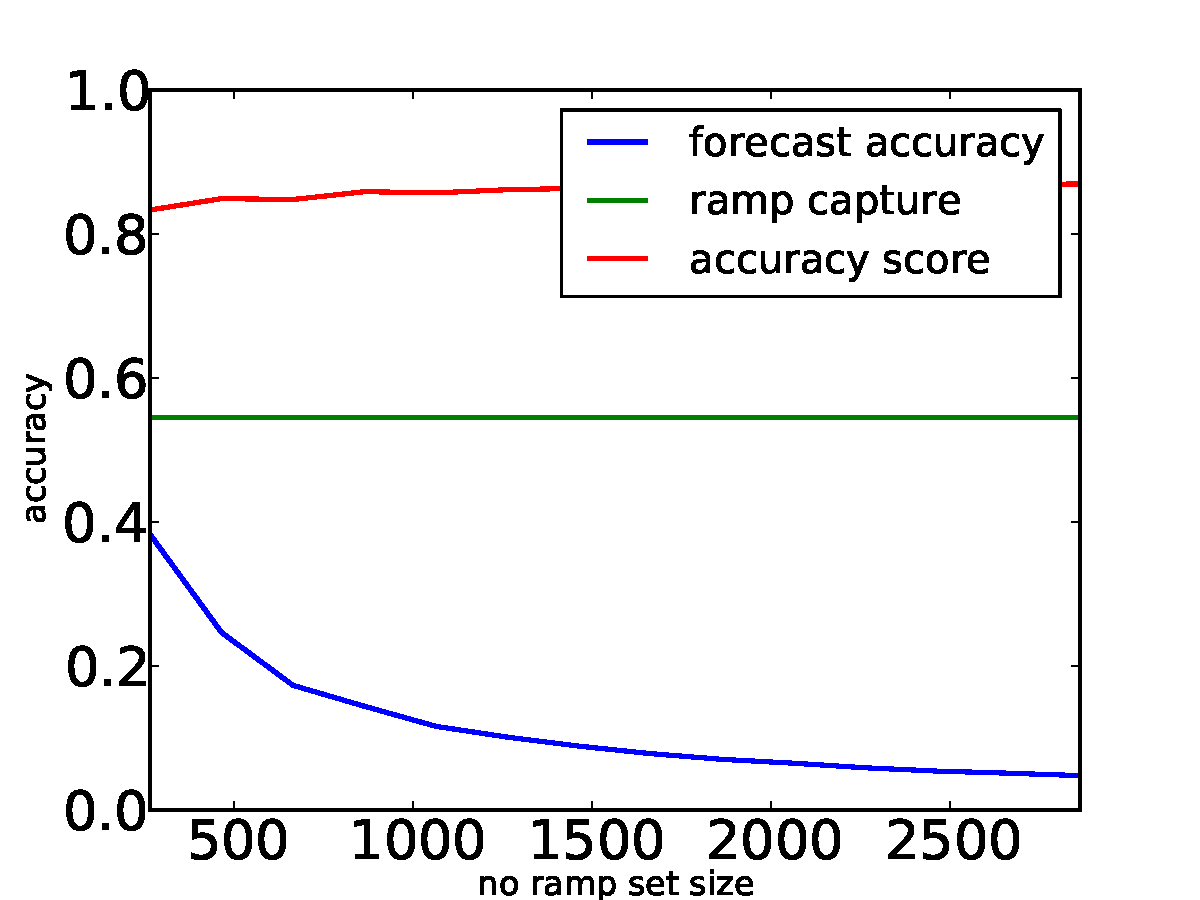
\includegraphics[scale=0.2]{pics/reno_test_h15_a1.pdf}}
\subfigure[Palm Springs, $\theta = 15, \alpha = 1$]{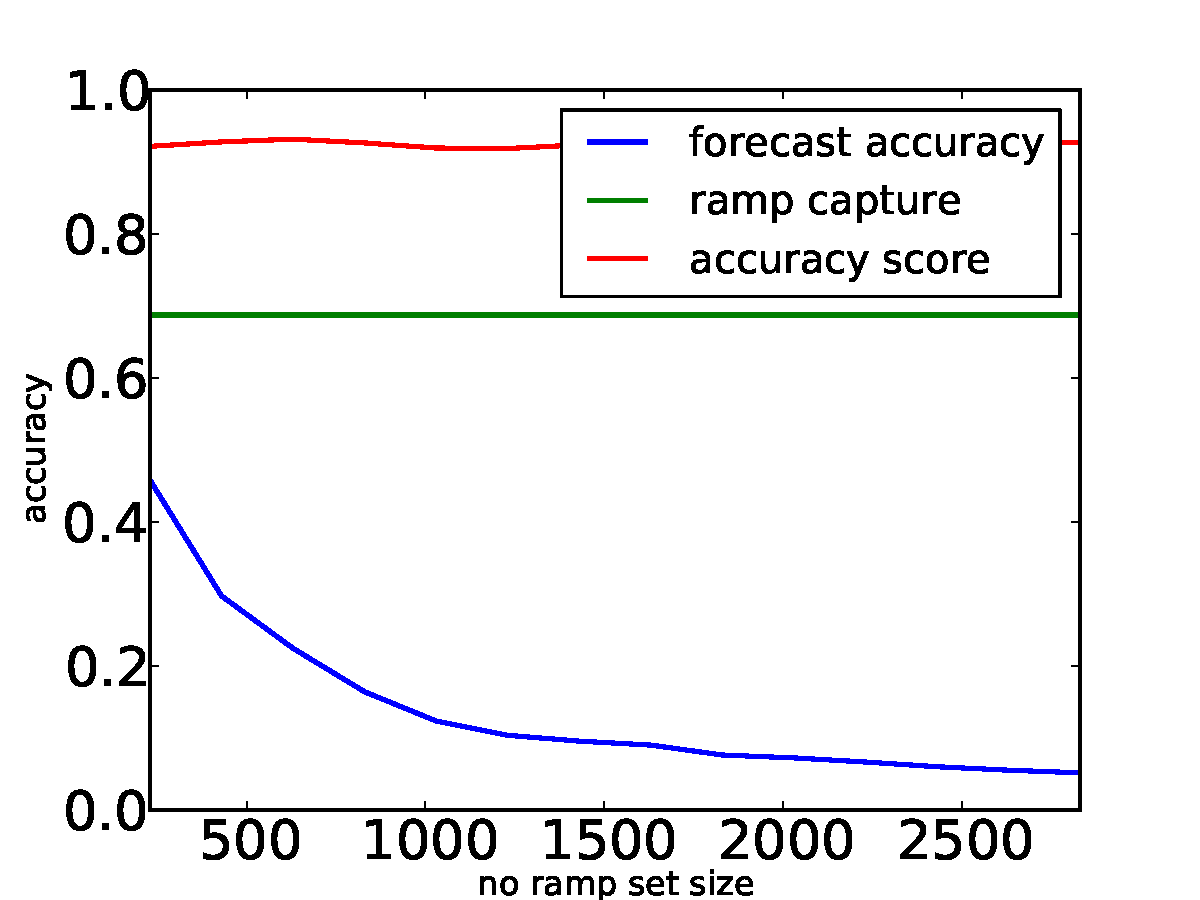
\includegraphics[scale=0.2]{pics/palm_test_h15_a1.pdf}}
\caption{SVM ramp prediction with balanced training set and test set with increasing number of no-ramp patterns for references turbines in (a) Reno and (b) Palm Springs ($\theta = 15, \alpha = 1$).}
\label{fig:unbalanced1}
\end{figure}

Figure~\ref{fig:unbalanced2} shows the result of SVM-based ramp event prediction w.r.t. a training set with increasing number of no-ramps. Here, we can observe that forecast accuracy $f_a$ and the ramp capture $r_c$ decrease with an increasing amount of no-ramps, while the accuracy score is even slightly increasing. But the forecast accuracy is still much better than in case of the balanced training set and increasing test set. The reason is that the classifier better learns to distinguish ramp-events from each other and from no-ramp events with more examples in the training set. But the cost that has to be paid is the ramp capture $r_c$, as the number of true forecasts $f_t$ decreases. 


\begin{figure}[thb]
\centering
\subfigure[Tehachapi, $\theta = 15, \alpha = 1$]{\includegraphics[scale=0.2]{pics/teha_train_h15_a1.pdf}}
\subfigure[Tehachapi, $\theta = 10, \alpha = 2$]{\includegraphics[scale=0.2]{pics/train_teha_h10_a2.pdf}}
\caption{SVM ramp prediction with unbalanced training sets, i.e., increasing number of no-ramp patterns in Tehachapi with (a) ($\theta = 15, \alpha = 1$) and (b) ($\theta = 10, \alpha = 2$).}
\label{fig:unbalanced2}
\end{figure}

The prediction of wind energy ramp events is a difficult undertaking. Although SVMs turn out to be comparatively strong classifiers, the achieved accuracy may not be high enough to avoid false alarms. The number of false positives is too large in case of a strongly unbalanced test data set situation. But this is usually the case in practical recognition scenarios as the number of no-ramps is about 150 to 300 times higher\footnote{We assume 10-minute time steps.} than the number of ramp events. Consequently, the accuracy of a classifier would have to exceed about $365/52560 \approx 0.995$ to allow at most one false alarm a day.



\section{Monitoring Module}
\label{sec:dimred}

Last, we introduce the monitoring module that allows to monitor high-dimensional wind time series. Monitoring is an important machine learning task in practical energy information system applications. Dimensionality reduction (DR) methods map high-dimensional patterns to low-dimensional representations. Often, sampling a subset of the data is not sufficient due to gradual changes in the time series. Varying weather conditions and seasonal changes are examples for such gradual changes in the wind time series data. 

In~\cite{neurocomp}, we employed self-organizing maps (SOMs) for sequence visualization of high-dimensional wind time series. Similar to vector quantization, SOMs learn to place codebook vectors in data spaces that can be used for visualization. The neurons can be employed for the assignment of patterns to colors, if neurons are assigned to colors, and neighbored neurons employ similar colors.  But the capabilities to visualize gradual changes of SOM-based monitoring is strongly restricted to the topology of the map, e.g., the number of neurons and the structure of the network (which is usually a simple lattice structure). The module allows the application of isometric mapping (ISOMAP)~\cite{isomap} and and locally linear embedding (LLE)~\cite{lle}. First, we show the results of embedding the high-dimensional patterns into 2-dimensional latent spaces. Then, we use the mapping into 3-dimensional latent spaces to colorize linear time series.


\subsection{Embeddings}

In the first step of our approach, the high-dimensional patterns are mapped to two-dimensional continuous latent spaces. To illustrate, how the results of this first step look like, we visualize the learning results for two-dimensional latent spaces. Figure~\ref{fig:isomap} shows the learning results of ISOMAP with (a) neighborhood size $K=10$ and (b) neighborhood size $K=30$. The data set employs $d=66$ wind turbines (grid points) in a radius of 10 km around a turbine in Tehachapi, California. Both embeddings show that ISOMAP and LLE are able to adapt to gradually changing wind situations. The embeddings employ colors according to the average wind power in the corresponding sequence.


\begin{figure}[h]
\begin{center}
\subfigure[ISOMAP, $K=10$]{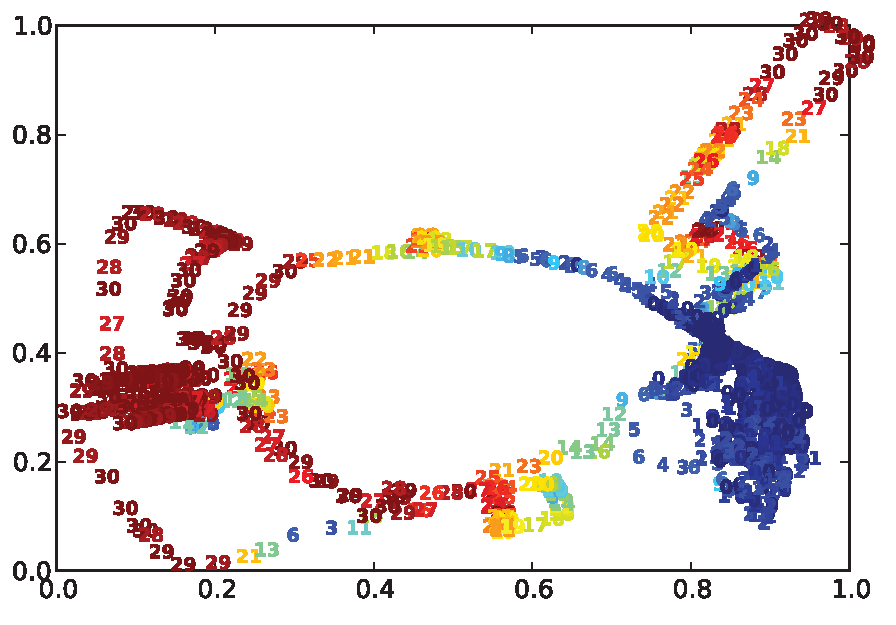
\includegraphics[scale=.27]{pics/isomap1.pdf}}
\subfigure[ISOMAP, $K=30$]{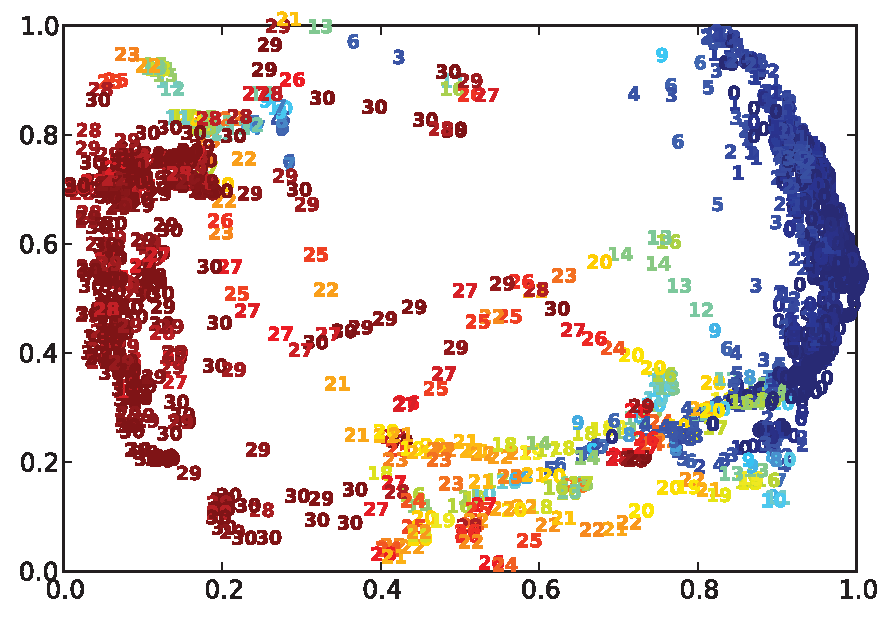
\includegraphics[scale=.27]{pics/isomap2.pdf}}
%\subfigure[ISOMAP, $K=30$]{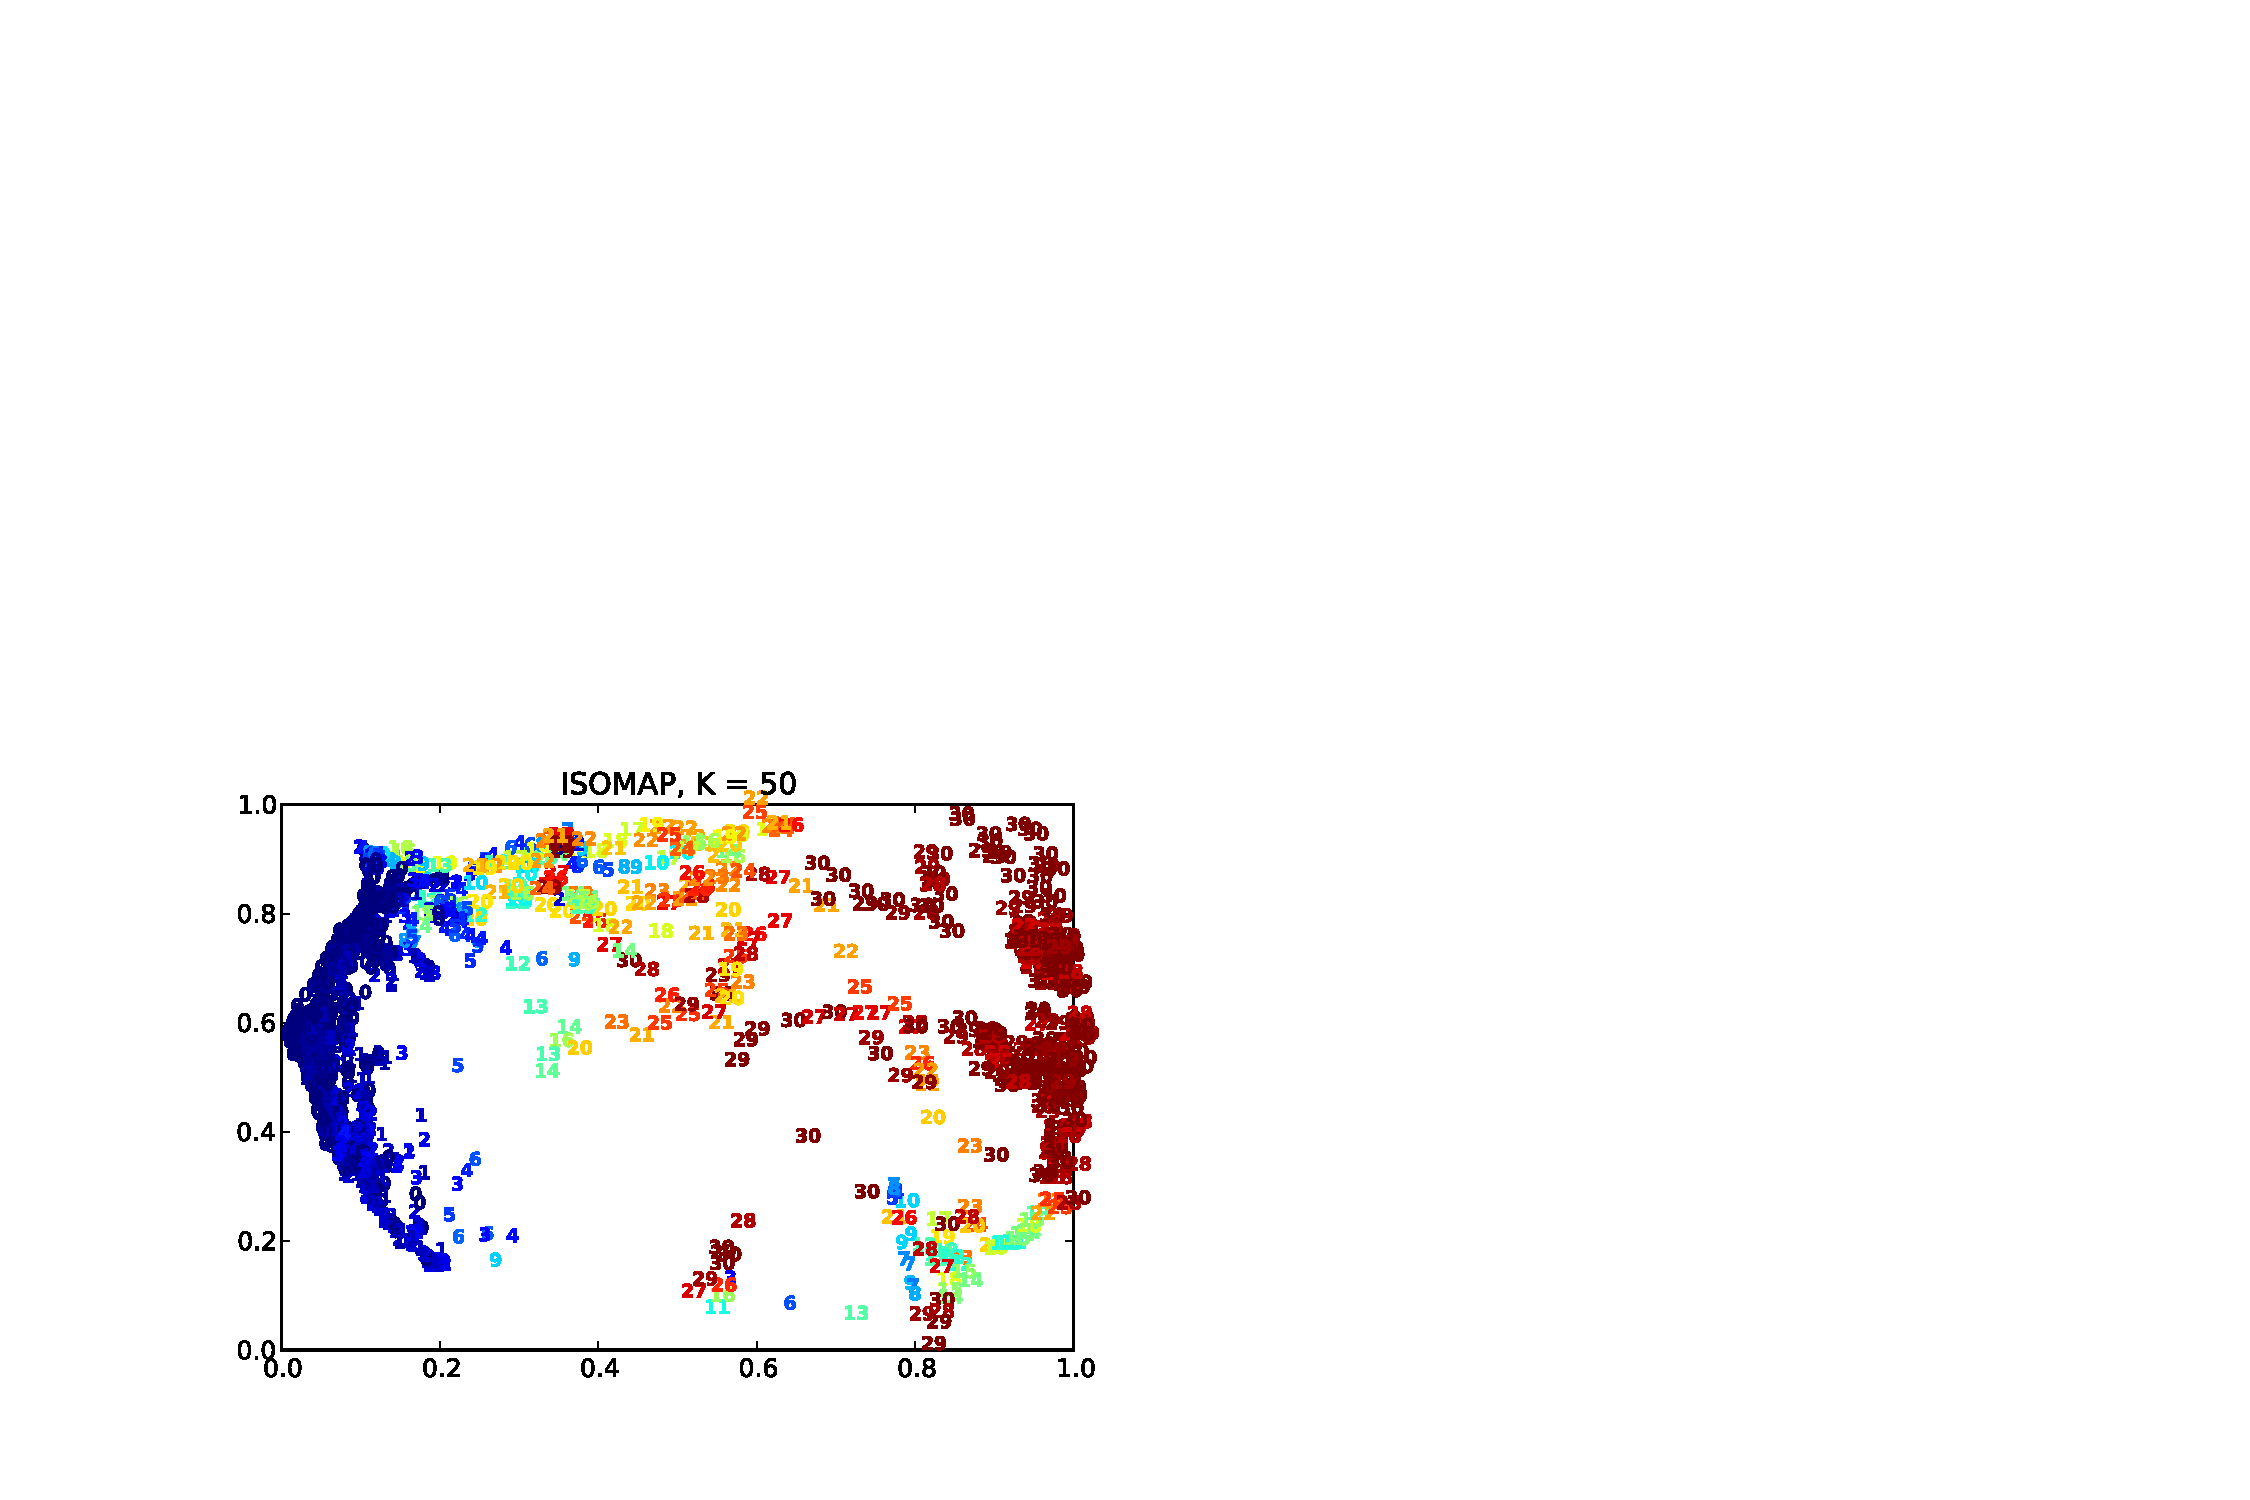
\includegraphics[scale=.29]{pics/iso3.pdf}}
\caption{\label{fig:isomap}Comparison of wind time series embeddings of ISOMAP for $N=1000$ $66$-dimensional wind energy time series patterns for $K=10$ and $K=30$.}
\end{center}
\end{figure}


\subsection{Monitoring}
\label{sec:mon}

In the following, we employ the learned manifold for visualization of wind time series in a test set. The latent positions of the trained manifold can be used for colorization of a horizontal bar over time of a test time series. In the test time series, pattern $\mathbf{y}_t$ of time step $t$ is assigned to the color 
\begin{figure}[h]
\begin{center}
\subfigure[ISOMAP, K=10]{\includegraphics[scale=.09]{pics/isomapk10a.pdf}}
\subfigure[ISOMAP, K=30]{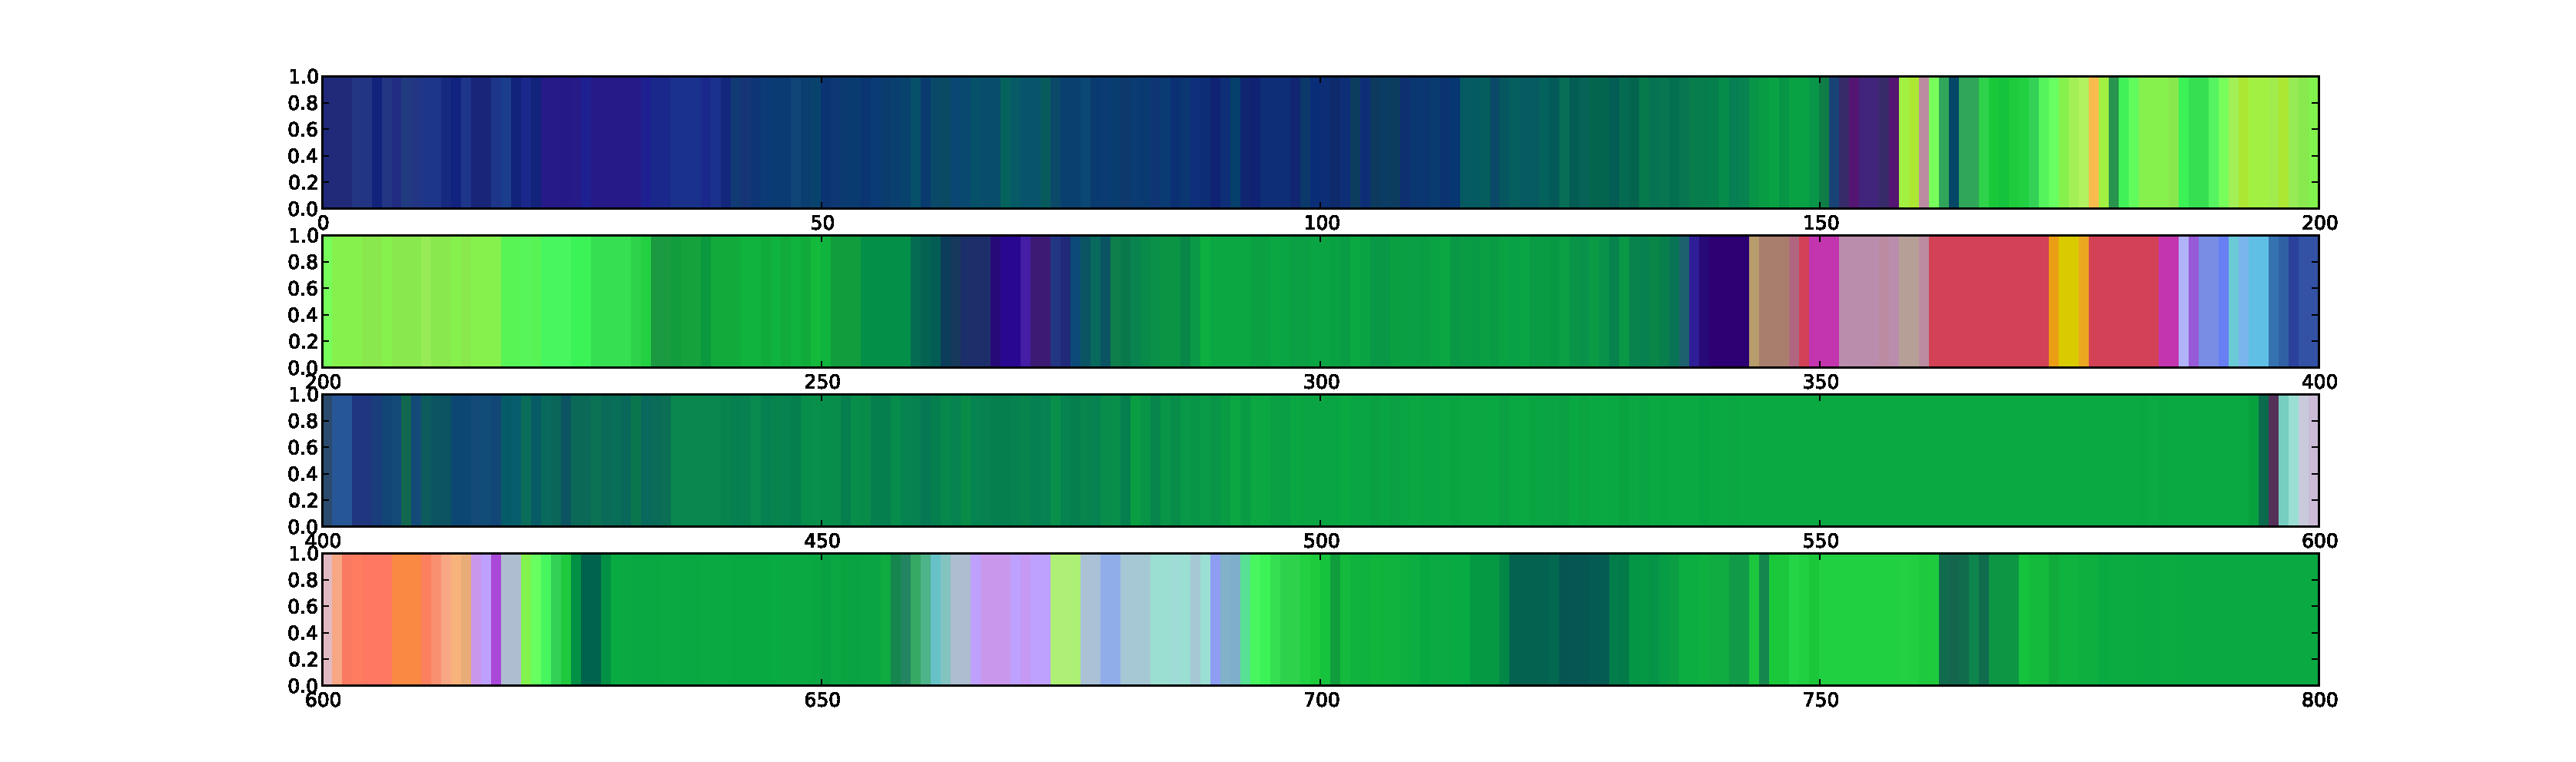
\includegraphics[scale=.09]{pics/isomapK30a.pdf}}
\subfigure[ISOMAP, K=50]{\includegraphics[scale=.09]{pics/isomapk50a.pdf}}
\subfigure[ISOMAP, K=100]{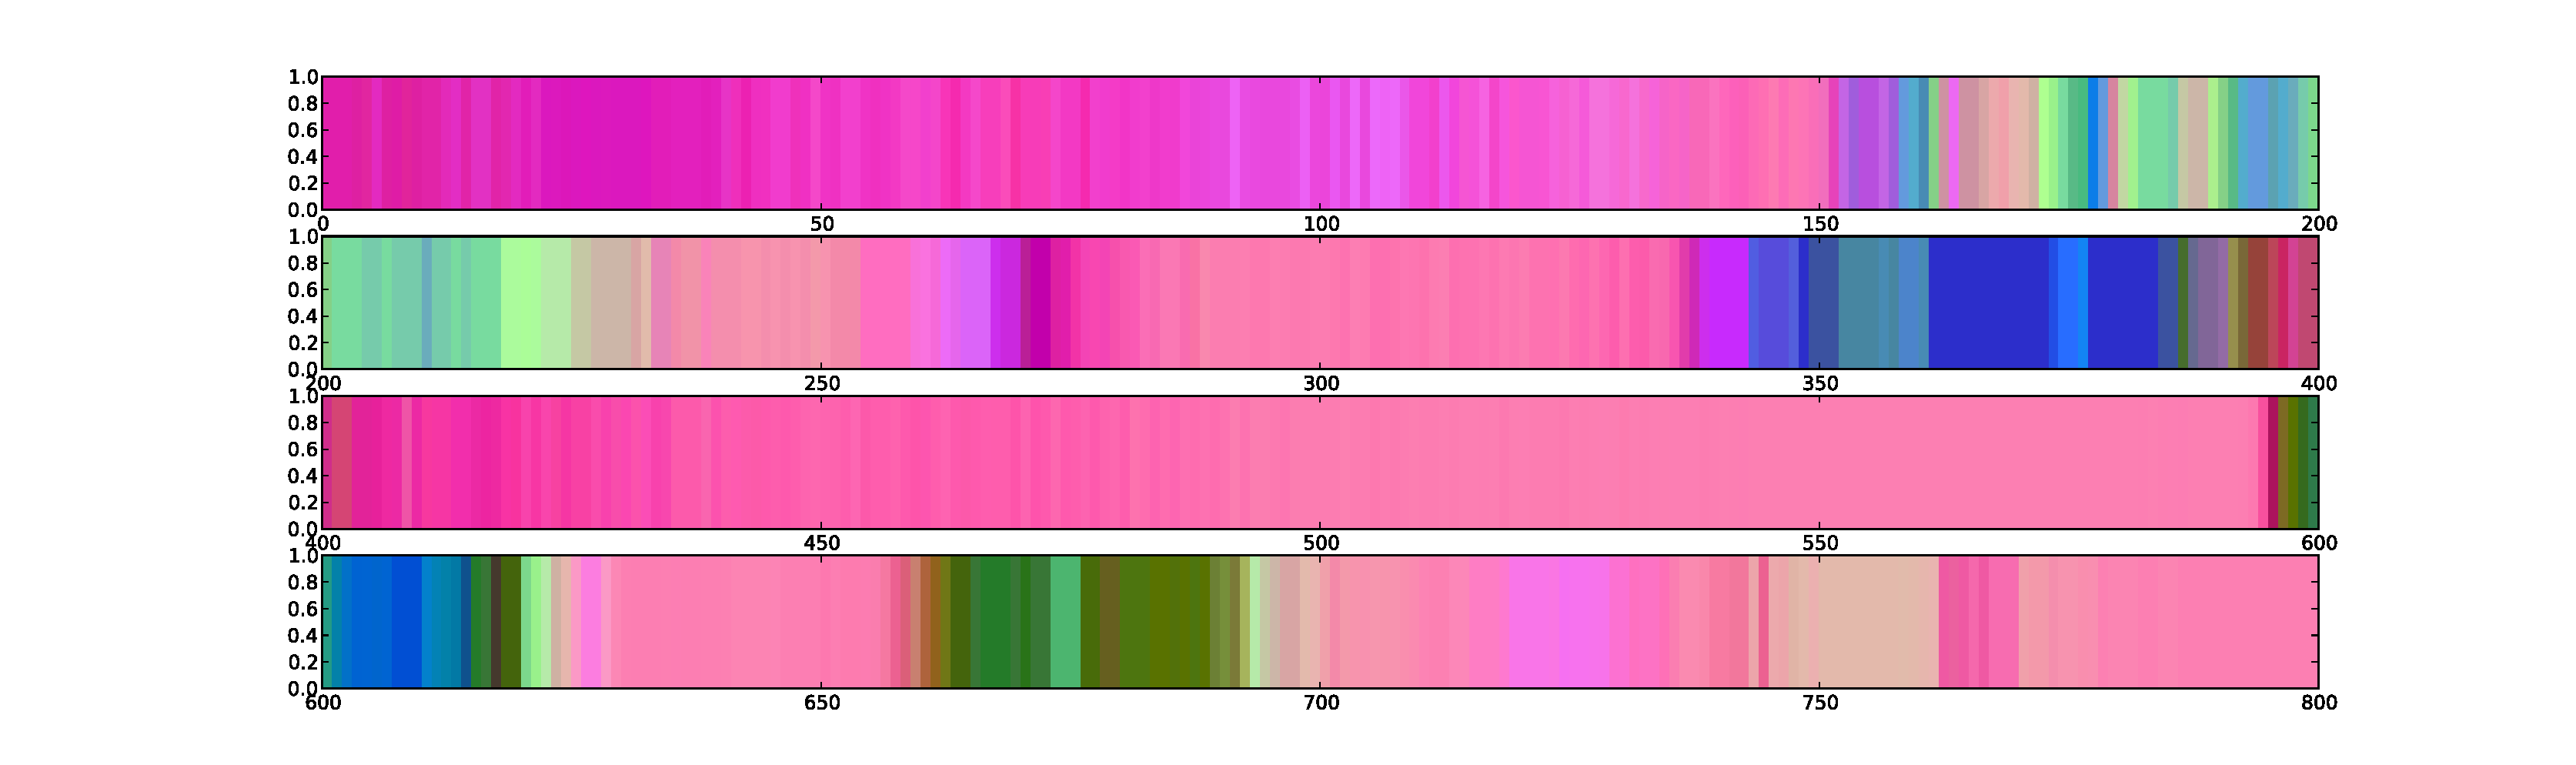
\includegraphics[scale=.09]{pics/isomapK100a.pdf}}
\subfigure[LLE, K=10]{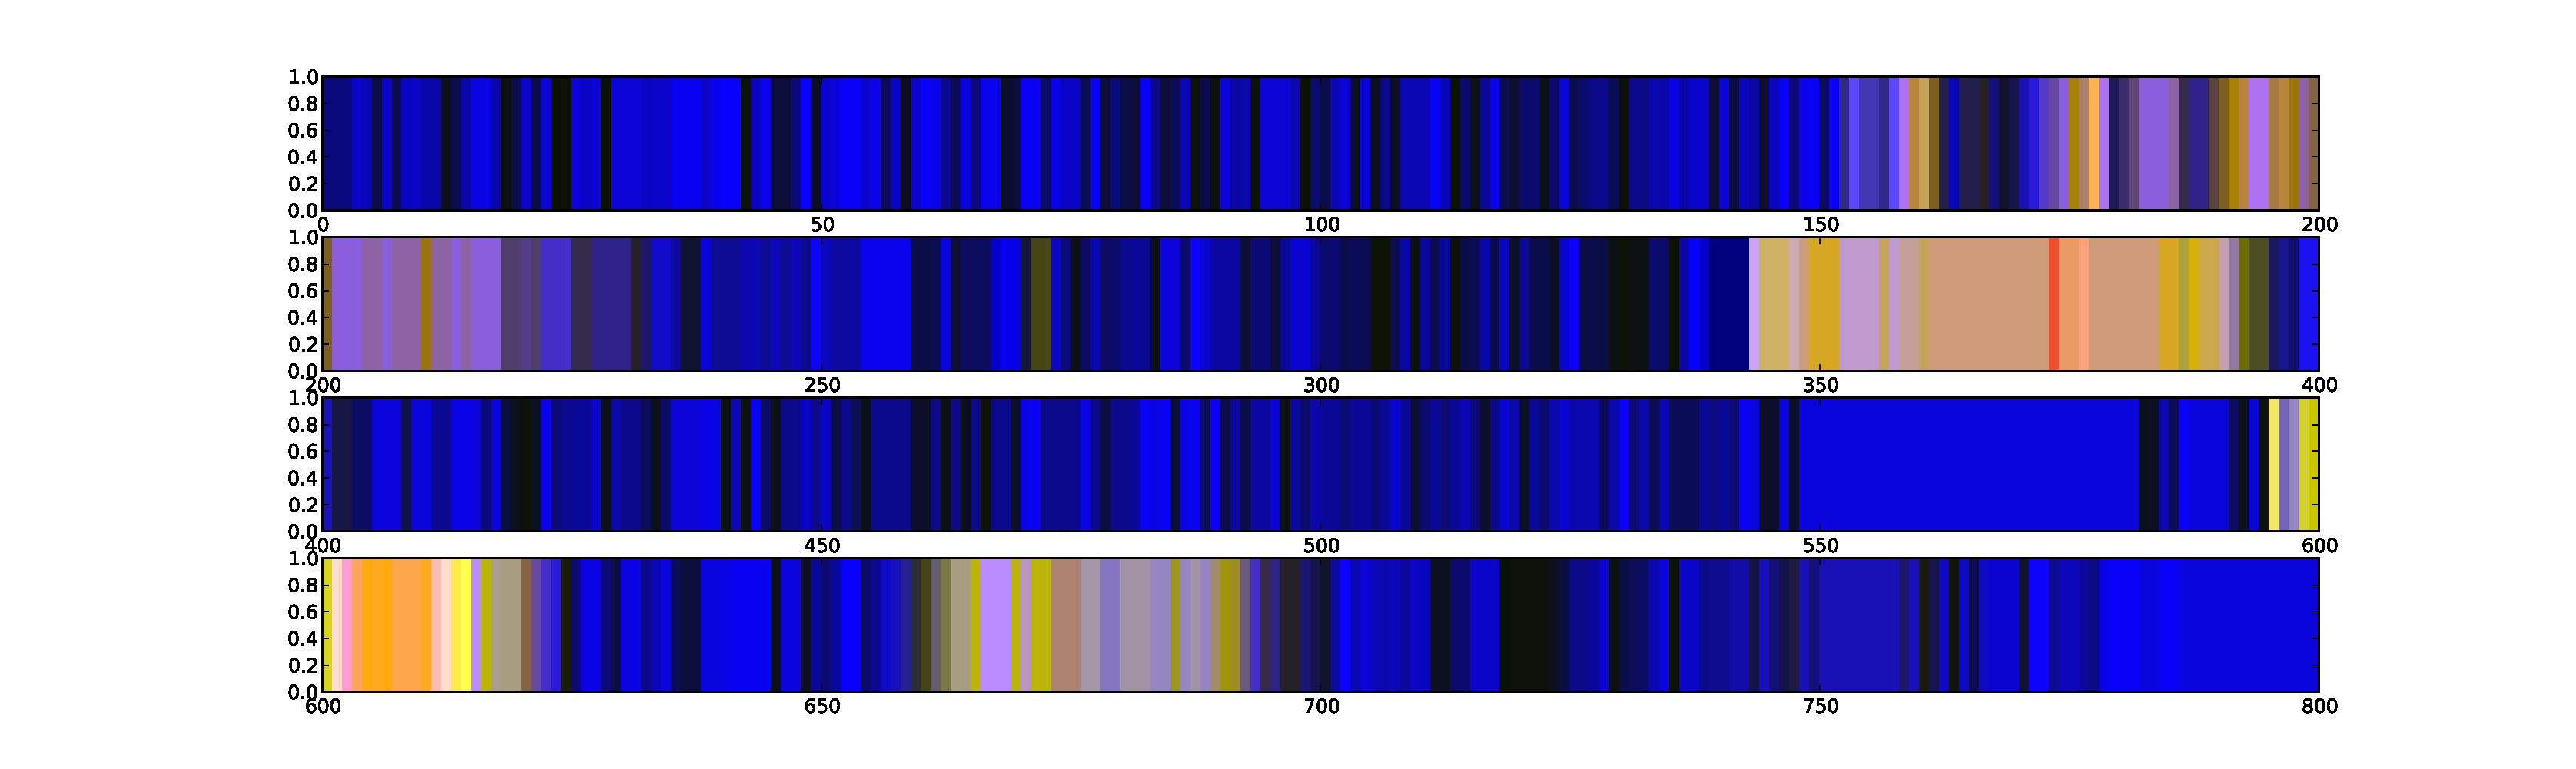
\includegraphics[scale=.09]{pics/llek10a.pdf}}
\subfigure[LLE, K=30]{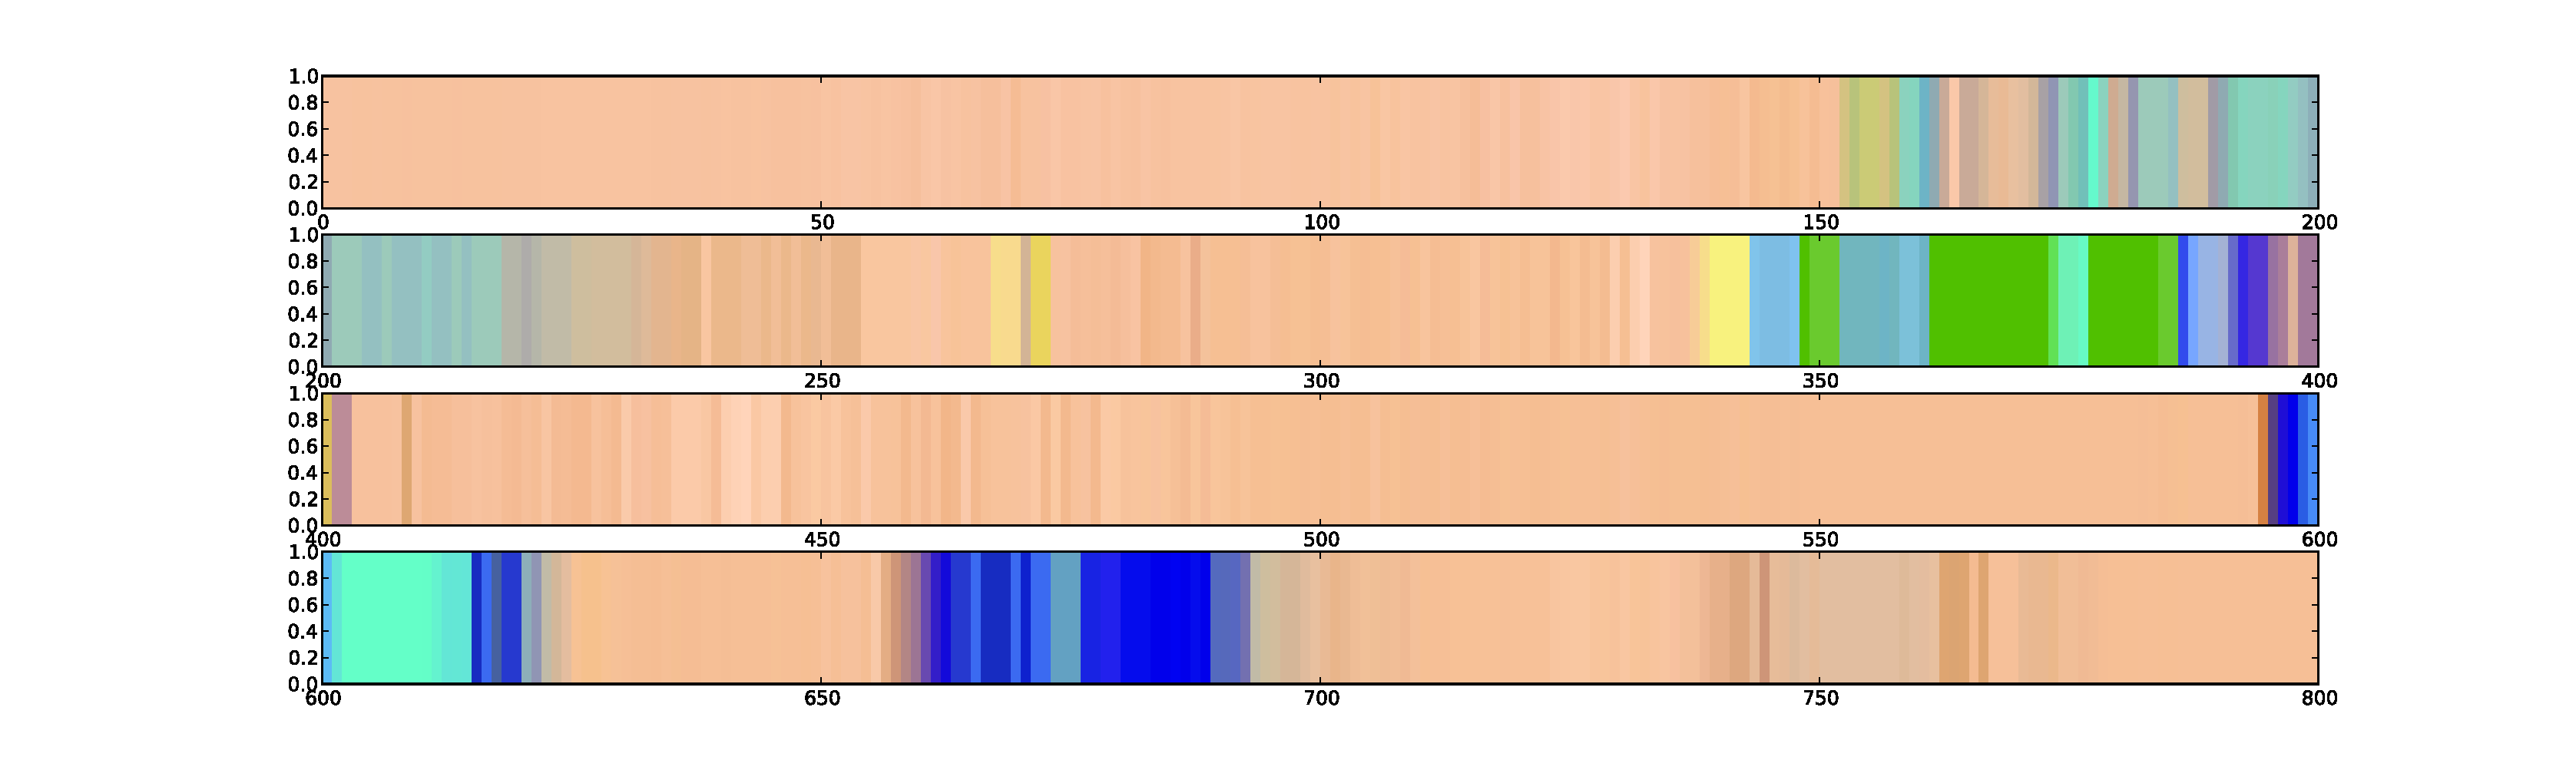
\includegraphics[scale=.09]{pics/lleK30a.pdf}}
\caption{\label{fig:monitor}Visualization of test sequence employing (a)+(b) ISOMAP and (c)+(d) LLE for $d=66$ turbines in Tehachapi.}
\end{center}
\end{figure}
that depends on the latent position $\mathbf{x}^*$ of its closest embedded pattern $\mathbf{y}*$ in the training manifold. For training, $N_1=2000$ time steps, i.e., patterns are used. We visualize a test set of $N_2=800$ steps in the following figures. Figure~\ref{fig:monitor} shows the monitoring results of ISOMAP with (a) $K=10$ and (b) $K=30$, as well as LLE with (c) $K=10$, and $K=30$. Areas colorized with a similar color and few color changes can be found in each case, while areas with frequent changes occur at the same locations in all plots. Both methods turn out to be robust w.r.t. the chosen neighborhood size $K$. The learning result of LLE with small neighborhood size $K=10$ is worse with unstable areas of fluctuating colors in stable not changing wind situations. 


\section{Conclusion}
\label{sec:cons}

Data mining in wind energy information systems is an excellent chance to increase the efficiency of integrating wind energy into smart grids. WindML is an easy-to-use python-based framework that allows an efficient design of wind energy application modules. The prediction modules for wind energy and ramp forecasts presented in this paper have an important part to play in practical applications of integrating wind energy into smart grids. With the regression module for wind power forecasting, we have introduced  the first systematic comparison of different regression techniques on the spatio-temporal time series prediction model. The classification module is the first approach for prediction of ramp events taking into account the spatio-temporal model emphasizing the problem of imbalanced data sets. The dimensionality reduction module extends our previous work by modules for embedding in continuous latent spaces.

A continuous extension of data mining tasks, the integration of further wind data sets and an adaptation to practical software packages for research and business applications are the future steps of WindML.



% conference papers do not normally have an appendix


% use section* for acknowledgement
\section*{Acknowledgment}

We thank the Pr\"{a}sidium of the Carl-von-Ossietzky University Oldenburg and the EWE research institute NextEnergy for partly supporting this work. Further, we thank NREL for the data sets of the western wind data set.



\bibliographystyle{abbrv}
\bibliography{literature}


% that's all folks
\end{document}

new results!
- ramp separation requires only one feature, logical!
- other results: ramp classification with no-ramps requires environment
- ramp classification with 3 classes is stronger than ramp classification with 2

known results:
- balanced training set deteriorates forecast accuracy on unbalanced test sets significantly due to increasing number of false forecasts
- training on imbalanced data sets weakens this argument (slower decrease of forecast accuracy), but deteriorates classifier (e.g. accuracy and rate of missed ramps)


questions:
- determine rate of turbines in selection problem, make plot like in sklearn
- can accuracy be improved with more "pasts"?
- how many features are required?
- comparison of classifiers
- combinatorial optimization
- comparison with regression approach: normal vs. height of change



